\chapter{Experiments}
\label{c:experiments}
\IMRADlabel{results}



In this chapter we will present all environments we experimented with as well as \emph{hyper-experiments}, \ie experiments with the hyperparameters and their influence on the algorithm performance (in terms of the prediction error and similar metrics, not the computing time).

We split this chapter into two parts: Firstly, we will present the experiment setup we used and the different environments we tested on. Secondly, we present our results and put them in context of other results. All critical discussion and comparison with related work will take place in~\autoref{c:discussion}.

\section{Setup}
	In this section we will introduce the experiment setup and all the different environments we used for evaluation.

	\subsection{Environments}
		This section covers the different environments we used and changes we have applied to them. Note that we separated the data generation process from running the experiment. For each of the following experiments we include the experiment ID at the beginning that can be used to locate the experiment in the code.

		\subsubsection{Proof-of-Concept: Classic LGDS}
			\begin{itemize}
				\item Experiment ID: \texttt{lgds}
			\end{itemize}

			As a proof-of-concept and to empirically verify our proof on the exactness of the cubature rule and hence the similar expected performance for plain linear systems, we benchmark our algorithm against a simple linear system. The linear system has a two-dimensional state \( \vec{y} \coloneqq \begin{bmatrix} x_1 & x_2 \end{bmatrix}^T \) with the dynamics
			\begin{align*}
				\dot{x}_1 &= x_2 \\
				\dot{x}_2 &= -x_1
			\end{align*}
			The initial state \( \vec{s}_1 \) is sampled from a Gaussian distribution with mean \( \begin{bmatrix} 0.1 & 0.2 \end{bmatrix}^T \) and covariance \( \diag\big(10^{-5}, 10^{-5}\big) \). The system is integrated using the implicit Runge-Kutta Radau~IIA~\cite{guglielmiImplementingRadauIIA2001} method with an evaluation interval of \( h = 0.1 \) for \( T = 240 \) time steps where only the first \( T_\train = 120 \) steps are used for training and the remaining \(120\) are used for validation.

			As the system's eigenvalues \( -i \), \( i \) are purely imaginary, the integrated system rings around the equilibrium \( \begin{bmatrix} 0 & 0 \end{bmatrix}^T \) indefinitely.
		% end

		\subsubsection{(Damped) Pendulum}
			\begin{itemize}
				\item Experiment ID: \texttt{pendulum} and \texttt{pendulum\_damped}
			\end{itemize}

			The first nonlinear system we look at is the (inverted) pendulum in both an undamped and a damped setting. For this experiment, we use the angular state \( \vec{y} = \begin{bmatrix} \theta & \dot{\theta} \end{bmatrix} \) where \(\theta\) is the displacement angle (see~\autoref{fig:simplePendulum}). The dynamics are specified by the \ac{ode}
			\begin{equation*}
				\ddot{\theta} = \sin\theta - d \dot{\theta}
			\end{equation*}
			that is solved using the Radau~IIA~\cite{guglielmiImplementingRadauIIA2001} \ac{ivp} integrator (after transforming the \ac{ode} to a first-order \ac{ode} system). The initial velocity is set to \(0\) and the initial position is sampled from a Gaussian distribution with mean \( \pi/36 \) and variance \( \pi/8 \). This puts the pendulum in motion as it falls down from its initial position. For the undamped pendulum, we set \( d = 0 \). For both environments, we use an evaluation interval of \( h = 0.1 \) for \( T = 1000 \) time steps where only the first \( T_\train = 500 \) steps are used for training and the remaining \(500\) are used for validation.

			The damped pendulum is especially interesting as the system looses energy (\ie the sum of the kinetic and potential energy decreases over time) and the embedding has to encode this behavior.
		% end

		\subsubsection{Gym Pendulum}
			\label{subsubsec:gymPendulum}

			\begin{itemize}
				\item Experiment ID: \texttt{pendulum\_gym}
			\end{itemize}

			This is a sine/cosine version of the pendulum introduced before, but without damping. We use the environment of OpenAI Gym~\cite{brockmanOpenAIGym2016} for generating the data used for training. The motion equations are still the same as for the non-Gym pendulum
			\begin{equation*}
				\ddot{\theta} = \sin\theta
			\end{equation*}
			with \( d = 0 \) as the Gym pendulum does not include damping, but the state is defined as the sine and cosine of the angle:
			\begin{equation*}
				\vec{y} \coloneqq
					\begin{bmatrix}
						\cos\theta \\
						\sin\theta \\
						\dot{\theta}
					\end{bmatrix}
			\end{equation*}
			The Gym environment uses the Euler method for integrating the \ac{ode} with a step size of \( h = 0.05 \). We generate \( T = 100 \) time steps of which \( T_\train = 50 \) are used for training and the other \(50\) for validation.
		% end

		\subsubsection{Gym Cartpole}
			\label{subsubsec:cartpole}

			\begin{itemize}
				\item Experiment ID: \texttt{cartpole\_gym}
			\end{itemize}

			The second to last environment we run experiment on is the cartpole environment. In the cartpole environment, an inverted pendulum is build on a (typically controlled, but otherwise freely movable) cart. If the pendulum falls down, the torque on the joint is translated into a force moving the cart around. This creates nonlinear coupling and therefore, highly nonlinear dynamics. A sketch of the cartpole environment is given in~\autoref{fig:envCartpoleGymSketch}. As for the previous pendulum, we rely on the cartpole implementation of Gym. We slightly modified the environment to be uncontrolled, as the environment usually has discrete actions for pushing the cart left or right. The state of the environment is given as
			\begin{equation*}
				\vec{y} \coloneqq
					\begin{bmatrix}
						x \\
						\dot{x} \\
						\theta \\
						\dot{\theta}
					\end{bmatrix}
			\end{equation*}
			where \(x\) is the cart position, \(\dot{x}\) is the cart velocity, \(\theta\) is the pole angle and \(\dot{\theta}\) is the angular velocity. The implemented equations of movement, taken from~\cite{florianCorrectEquationsDynamics2005}, are given as:
			\begin{align*}
				\ddot{\theta} &= \frac{g \sin\theta + \cos\theta \Big(\! \frac{-F - m_p \ell \dot{\theta}^2 \sin\theta}{m_c + m_p} \!\Big)}{\ell \Big(\! \frac{4}{3} - \frac{m_p \cos^2\theta}{m_c + m_p} \!\Big)} \\
				\ddot{x} &= \frac{F + m_p \ell \big( \dot{\theta}^2 \sin\theta - \ddot{\theta} \cos\theta \big)}{m_c + m_p}
			\end{align*}
			Here \( g = \SI{9.8}{\meter\per\second\squared} \) is the gravitational acceleration, \( m_p = \SI{0.1}{\kilogram} \) and \( m_c = \SI{1}{\kilogram} \) are the masses of the pole and cart, respectively, \( 2\ell = \SI{1}{\meter} \) is the pole length and \( [F] = \si{\newton} \) is the external (control) force acting on the cart that we set to \( \SI{0}{\newton} \). The Gym environment uses an implicit Euler method for integrating the \ac{ode} with a step size of \( h = 0.02 \). We generate \( T = 300 \) time steps of which we use \( T_\train = 150 \) for training and the remaining \(150\) steps for validation.

			\begin{figure}
				\centering
				\tikzCartpole
				\caption[Illustration of the cartpole environment]{Illustration of the cartpole environment. The cart has mass \(m_c\), the pole \(m_p\) with length \(L\). The cart can move freely on the \(x\) axis, while the pendulum can swing freely around the center of the cart, causing the cart to move.}
				\label{fig:envCartpoleGymSketch}
			\end{figure}
		% end

		\subsubsection{Gym Double Pendulum}
			\label{subsubsec:doublePendulum}

			\begin{itemize}
				\item Experiment ID: \texttt{acrobot\_gym}
			\end{itemize}

			The last environment we test on is the double pendulum, implemented in Gym as the \emph{acrobot} (as for the cartpole, we removed all control inputs and modified the initial state to start on top rather than hanging straight down). The double pendulum consists of a pendulum on a fixed joint and a second pendulum attached to the end of the first pendulum. This creates highly nonlinear coupling and is the most common example of a chaotic system~\cite{shinbrotChaosDoublePendulum1992}. We observe the state vector
			\begin{equation*}
				\vec{y} \coloneqq
					\begin{bmatrix}
						\cos\varphi_1 \\
						\sin\varphi_1 \\
						\cos\varphi_2 \\
						\sin\varphi_2 \\
						\dot{\varphi}_1 \\
						\dot{\varphi}_2
					\end{bmatrix}
			\end{equation*}
			where \(\varphi_1\) and \(\varphi_2\) are the displacement of the first and second joint, respectively. See~\autoref{fig:envDoublePendulumGymSketch} for a sketch of the double pendulum. The governing equations of motion are given as:
			\begin{align*}
				\ddot{\varphi}_1 &= \frac{g (\sin\varphi_2 \, \cos\varphi_\Delta - \mu \sin\varphi_1) - (\ell_2 \dot{\varphi}_2^2 + \ell_1 \dot{\varphi}_1^2 \cos\varphi_\Delta) \sin\varphi_\Delta}{\ell_1 (\mu - \cos^2\varphi_\Delta)} \\
				\ddot{\varphi}_2 &= \frac{g \mu (\sin\varphi_2 \, \cos\varphi_\Delta - \mu \sin\varphi_1) + (\mu \ell_1 \dot{\varphi}_1^2 + \ell_2 \dot{\varphi}_2^2 \cos\varphi_\Delta) \sin\varphi_\Delta}{\ell_2 (\mu - \cos^2\varphi_\Delta)}
			\end{align*}
			with \( \varphi_\Delta \coloneqq \varphi_1 - \varphi \), \( \mu \coloneqq 1 + m_1/m_2 \) where \( g = \SI{9.8}{\meter\per\second\squared} \) is the gravitational acceleration, \( m_1 = \SI{1}{\kilogram} \) and \( m_2 = \SI{1}{\kilogram} \) are the masses of the two links and \( \ell_1 = \SI{1}{\meter} \) and \( \ell_2 = \SI{1}{\meter} \) are the lengths of the two links. The Gym environment uses a \ac{rk4} for integrating the \ac{ode} with an evaluation interval of \( h = 0.2 \). We modified the initial position to be drawn from a Gaussian distribution with mean \( \pi \) and standard deviation \( \pi/8 \) and the initial velocity to be drawn from a uniform distribution in the interval \( [-0.1, 0.1] \). We generate \( T = 75 \) time steps of which we use \( T_\train = 56 \) (\(75\%\)) for training and the remaining \(19\) for validation.

			\begin{figure}
				\centering
				\tikzDoublePendulum
				\caption[Illustration of the double pendulum environment]{Illustration of the double pendulum environment. The pendulums have lengths \(\ell_1\) and \(\ell_2\) with the masses \(m_1\) and \(m_2\) attached to the respective ends. The inner pendulum can swing freely around the center while the other pendulum can swing freely around the end of the inner pendulum. Hence, fixing one of the pendulums would transform the system back to a simple pendulum. If both pendulums can swing, the system is chaotic.}
				\label{fig:envDoublePendulumGymSketch}
			\end{figure}
		% end
	% end

	\subsection{Experiment Setup}
		\label{subsec:experimentSetup}

		We now introduce the experiment setup and initialization we used for each environment. For all experiments, we initialized the latent state dynamics matrix \( \mat{A} \) with an identity matrix, the initial state \( \vec{m}_0 \) with a one-vector and all covariance matrices \( \mat{R} \), \( \mat{Q} \) and \( \mat{V}_0 \) with a small diagonal covariance of \( 10^{-5} \). We set the maximum number of \(\vec{g}\)-optimization iterations to \(1000\) for all environments. As described in~\autoref{sec:implementation}, we used a neural network for the observation function with \(\tanh\) activation functions (except for the output layer of course) and a single hidden layer with \(50\) neurons. We used \(100\) maximum iterations for the pendulum, \(200\) for the damped pendulum, \(500\) for the Gym pendulum, \(500\) for the Gym cartpole and \(250\) for the Gym double pendulum.

		For the proof-of-concept environment (the linear system), we used a slightly different setup as the environment is a lot simpler. We used a zero-layer neural network with no activation function, \ie a learnable matrix/linear transformation. We also fixed the latent dimensionality to be \(2\) for the linear system as we only have two states.
	% end

	\subsection{Hyper-Experiments}
		Besides the performance on specific environments, we were interested in how hyperparameters like the latent dimensionality affect the performance of the system. In this section we will discuss and present our experiment setup for the "hyper-experiments". All hyperparameters that are not part of the experiment where set as in in~\autoref{subsec:experimentSetup}.

		If not stated differently, we always ran the experiment with five different seeds to average out initialization noise.

		\subsubsection{Influence of the Latent Dimensionality}
			\label{subsec:experimentLatentDim}

			As the latent dimensionality directly influences how well the Koopman matrix can approximate the infinite-dimensional operator, it is one of the most interesting hyperparameters we evaluate. Hence, we evaluate multiple different latent dimensionalities from \( k = 1 \) to \( k = 50 \).
		% end
	% end
% end

\section{Results}
	\label{sec:results}

	In this section we will look at the results of the experiments described above. We organized the section into the different environments and will take a look at both the hyper-experiments first and then the individual results for optimized hyperparameters.

	For evaluating the performance of the model, we use different measures and metrics, both qualitative and quantitative. For a qualitative evaluation, we simply plot the produced data. These plots can get quite noisy as we will see, but they comprise all things we need for a qualitative assessment:
	\begin{itemize}
		\item The \emph{ground truth}, generated as described above with the adequate numerical integration of the equations of motion.
		\item The \emph{smoothed states} as they are produced from the E-step of the \algname algorithm, \ie \(\hat{\vec{s}}_{1:T}\).
		\item The \emph{rollout}, starting both from the learned initial value as well as from the last smoothed state. While the former visualizes the ability of the model to work completely "on its own", the latter shows how well the linear dynamics generalize beyond the training data.
		\item And of course the confidence (\ie the learned variance) around each trajectory.
	\end{itemize}
	For quantitative comparison, we focus on the \ac{nrmse} across all dimensions and time steps, computed as
	\begin{equation*}
		\mathit{NRMSE} = \frac{1}{k} \sum_{i = 1}^{k} \frac{1}{y_\mathrm{max} - y_\mathrm{min}} \sqrt{ \frac{1}{T} \sum_{t = 1}^{T} (y_{t, i} - \tilde{y}_{t, i})^2 }
	\end{equation*}
	where \( y_{t, i} \) is the true data and \( \tilde{y}_{t, i} \) is the corresponding data to evaluate at the \(t\)-th time step of the \(i\)-th dimension. We can compute four different error values: The error over the rollout from start to finish (\( t = 1, 2, \rangedots, T \)), over the training data only (\( t = 1, 2, \rangedots, T_\train \)), over the prediction only (\( t = T_\train, T_\train + 1, \rangedots, T \)) or over the smoothed trajectory (\ie the results from the E-step, \(  \hat{\vec{s}}_{1:T} \)). The latter primarily checks that our algorithm performs correct and that it is even capable of learning the dynamics and it should be near zero or at least below one for a decent parameter choice and model performance. On the other hand, the \ac{nrmse} over the complete rollout describes the generalization abilities. In conjunction with the rollout error over the training and prediction set, we can see which rollout primarily caused the complete error. We expected a low error on the training set for every environment.

	Using the \ac{nrmse} instead of the plain \ac{rmse} allows us to compare model performance across the difference dimensions as we are scaling the error to a reasonable interval. For error values below \( 0.01 \), we say that the error is close to zero as it only deviates at most \(1\%\) from the true data. For \(<0.1\) we say it is a good fit, and for \(<0.2\) we say the approximation is decent. However, we have to take these numbers with care as they summarize a lot of data into a single scalar.

	All subsections (of non-proof-of-concept environments) are separated into two main parts: Looking at the hyper-experiment of the latent dimensionality and inspect how well the model performs with different latent dimensionalities. Then we will pick two or three of those latent dimensionalities and look at the qualitative plots of the runs (exemplary evaluation).

	Each exemplary evaluation also contains the ID of the run containing the data we used and the raw data of the runs is added to the \hrefGithubKoopmanInference{GitHub repository} along with the code. The documentation for how to generate the plots is also there.

	\subsection{Proof-of-Concept: LGDS}
		For the \ac{lgds} environment, we did not run multiple latent dimensionalities as we already know how many states we have.~\autoref{fig:lgdsRollout} shows the rollout plot for \( k = 3 \) latent dimensions. As expected, both the rollout and the smoothed states perfectly match the true data, even in the prediction time span.

		\begin{figure}
			\centering
			\includegraphics[width=\linewidth]{figures/results/lgds/rollout-observations-N0.png}
			\caption[Rollout of the proof-of-concept LGDS experiment for 3 latent dimensions]{The rollout plot in the observation space of the LGDS environment for \(k = 3\). The left plot shows the first dimension, the right plot the second dimension. The black dots represent the true data of which the model used everything till the red prediction boundary to train on. The blue line is the rollout, starting from the learned initial value (marked with a green star). The orange dash-dotted line is the smoothed data. The dotted orange line then is the rollout starting from the last smoothed state, forming the "smoothed prediction". The orange lines are directly behind the blue ones, hence they are not visible. The shaded regions show the confidence, \ie two times the standard deviation.}
			\label{fig:lgdsRollout}
		\end{figure}
	% end

	\subsection{Pendulum} % TODO: Maybe update with results from GPU…
		\subsubsection{Influence of the Latent Dimensionality}
			For the pendulum experiment, we tested \(50\) latent dimensionalities from \( k = 1 \) to \( k = 50 \).

			We start by having a first look at the \ac{nrmse} of the smoothed trajectory in~\autoref{fig:pendulumRmseSmoothed} to see how many latent dimensions we need at least to get a model that is even slightly capable of learning the pendulum dynamics. We see that the \ac{nrmse} shrinks to near zero (less than \( 0.01 \)). Even for \( k = 1 \), the error is only approximately \( 0.18 \).

			\begin{figure}
				\centering
				\includegraphics[width=0.7\linewidth]{figures/results/pendulum-damped/latent-dim/comparison-rmse-smoothed-normalized-mean-vs-latent-dim.png}
				\caption[Error of the smoothed trajectory on the training data of the pendulum experiment]{The NRMSE of the smoothed trajectory on the training data of the pendulum environment.}
				\label{fig:pendulumRmseSmoothed}
			\end{figure}

			Looking at the \ac{nrmse} of the complete rollout in~\autoref{fig:pendulumRmseComplete}, we see that the error is quite noisy due to initialization. Nevertheless, the error shrinks until \( k \geq 10 \) and then stabilizes around an error of approximately \(0.15\). Comparing the complete rollout error with the training and prediction \ac{nrmse} in~\autoref{fig:pendulumRmseTrain} and~\autoref{fig:pendulumRmsePred}, respectively, we see that the training error falls until \( k \geq 10 \) and then stabilizes around \(0.08\). For the prediction error, we see a similar connection to \( k \geq 10 \), but the error does not shrink as much and always is around \(0.20\).

			\begin{figure}
				\centering
				\begin{subfigure}{0.7\linewidth}
					\centering
					\includegraphics[width=\linewidth]{figures/results/pendulum/latent-dim/comparison-rmse-rollout-normalized-mean-vs-latent-dim.png}
					\caption[Error of the complete rollout on the pendulum environment]{Error of the complete rollout on the pendulum environment.}
					\label{fig:pendulumRmseComplete}
				\end{subfigure} \\
				\begin{subfigure}{0.5\linewidth}
					\centering
					\includegraphics[width=\linewidth]{figures/results/pendulum/latent-dim/comparison-rmse-rollout-train-normalized-mean-vs-latent-dim.png}
					\caption[Error of the training rollout on the pendulum environment]{Error of the rollout on the training data only on the pendulum environment.}
					\label{fig:pendulumRmseTrain}
				\end{subfigure}%
				~
				\begin{subfigure}{0.5\linewidth}
					\centering
					\includegraphics[width=\linewidth]{figures/results/pendulum/latent-dim/comparison-rmse-rollout-prediction-normalized-mean-vs-latent-dim.png}
					\caption[Error of the prediction rollout on the pendulum environment]{Error of the rollout on the prediction only on the pendulum environment.}
					\label{fig:pendulumRmsePred}
				\end{subfigure}
				\caption[Errors on the pendulum environment for different latent dimensions]{Plot of the errors of the pendulum environment for different latent dimensions. The black dots show the measured data, the blue line the average of the data points for a specific latent dimensionality. The blue shaded region shows two times the standard deviation.}
				\label{fig:pendulumRmse}
			\end{figure}
		% end

		\subsubsection{Exemplary Evaluation: 2-Dimensional Latent}
			We now look at an exemplary run for the latent dimensionality \( k = 2 \) (run \texttt{100}). Looking at the errors, the rollout trajectory should be off the real data, but the smoothed trajectory should nearly match the true data.~\autoref{fig:pendulumRolloutL02} shows that the rollout and also the rollout of the smoothed trajectory are far off with low confidence, but the true data is in the confidence region. However, the smoothed trajectory follows the true data really good.
		% end

		\subsubsection{Exemplary Evaluation: 10-Dimensional Latent}
			\label{subsubsec:pendulumL10}

			We now look at an exemplary run for the latent dimensionality \( k = 10 \) (run \texttt{10}) as we postulated from the \ac{nrmse} data that this is the boundary, after which we expected diminishing returns.~\autoref{fig:pendulumRolloutL10} shows the rollout of the model, where the dynamics of the system are captured quite well with high confidence. Also the prediction is good, so that the differences between true data, smoothed prediction and rollout are small.

			\begin{figure}[H]
				\centering
				\includegraphics[width=\linewidth]{figures/results/pendulum/run-latent-dim-10/rollout-observations-N0.png}
				\caption[Rollout of the pendulum experiment for 10 latent dimensions]{The rollout plot in the observation space of the pendulum environment for \(k = 10\). The left plot shows the displacement and the right plot the angular velocity. The black dots represent the true data of which the model used everything till the red prediction boundary to train on. The blue line is the rollout, starting from the learned initial value (marked with a green star). The orange dash-dotted line is the smoothed data. The dotted orange line then is the rollout starting from the last smoothed state, forming the "smoothed prediction". The shaded regions show the confidence, \ie two times the standard deviation.}
				\label{fig:pendulumRolloutL10}
			\end{figure}
		% end

		\subsubsection{Exemplary Evaluation: 14-Dimensional Latent}
			\label{subsubsec:pendulumL14}

			We now look at an exemplary run for the latent dimensionality \( k = 14 \) (run \texttt{210}) for which we got the smallest overall \ac{nrmse}.~\autoref{fig:pendulumRolloutL14} shows the rollout of the model. In comparison to the 10-dimensional latent, nothing has changed, fulfilling the expectation of diminishing returns with high latent dimensionality.
		% end
	% end

	\subsection{Damped Pendulum} % TODO: Maybe update with results from GPU…
		\subsubsection{Influence of the Latent Dimensionality}
			For the damped pendulum experiment, we tested \(50\) latent dimensionalities from \( k = 1 \) to \( k = 50 \).

			We start by having a first look at the \ac{nrmse} of the smoothed trajectory in~\autoref{fig:pendulumDampedRmseSmoothed} to see how many latent dimensions we need at least to get a model that is even slightly capable of learning the damped pendulum dynamics. We see that the \ac{nrmse} shrinks to near zero (less than \( 0.01 \)) for latent dimensionalities of \( k \geq 2 \). Even for \( k = 1 \), the error is only approximately \( 0.09 \).

			Looking at the \ac{nrmse} of the complete rollout in~\autoref{fig:pendulumDampedRmseComplete}, we see that there is a point of diminishing returns in terms of the latent dimensionality for \( k \geq 10 \), where we get decent errors (around \( 0.05 \)) for all latent dimensionalities. Looking at the parts the complete \ac{nrmse} is composed of, the training and prediction error in~\autoref{fig:pendulumDampedRmseTrain} and~\autoref{fig:pendulumDampedRmsePred}, respectively, we see that the latent dimensionality affects both parts, the training and prediction error. However, the prediction error is generally smaller, which is mostly caused by the value of the state and hence the rollout being smaller.

			\begin{figure}
				\centering
				\includegraphics[width=0.7\linewidth]{figures/results/pendulum-damped/latent-dim/comparison-rmse-smoothed-normalized-mean-vs-latent-dim.png}
				\caption[Error of the smoothed trajectory on the training data of the damped pendulum experiment]{The NRMSE of the smoothed trajectory on the training data of the damped pendulum environment.}
				\label{fig:pendulumDampedRmseSmoothed}
			\end{figure}

			\begin{figure}
				\centering
				\begin{subfigure}{0.7\linewidth}
					\centering
					\includegraphics[width=\linewidth]{figures/results/pendulum-damped/latent-dim/comparison-rmse-rollout-normalized-mean-vs-latent-dim.png}
					\caption[Error of the complete rollout on the damped pendulum environment]{Error of the complete rollout on the damped pendulum environment.}
					\label{fig:pendulumDampedRmseComplete}
				\end{subfigure} \\
				\begin{subfigure}{0.5\linewidth}
					\centering
					\includegraphics[width=\linewidth]{figures/results/pendulum-damped/latent-dim/comparison-rmse-rollout-train-normalized-mean-vs-latent-dim.png}
					\caption[Error of the training rollout on the damped pendulum environment]{Error of the rollout on the training data only on the damped pendulum environment.}
					\label{fig:pendulumDampedRmseTrain}
				\end{subfigure}%
				~
				\begin{subfigure}{0.5\linewidth}
					\centering
					\includegraphics[width=\linewidth]{figures/results/pendulum-damped/latent-dim/comparison-rmse-rollout-prediction-normalized-mean-vs-latent-dim.png}
					\caption[Error of the prediction rollout on the damped pendulum environment]{Error of the rollout on the prediction only on the damped pendulum environment.}
					\label{fig:pendulumDampedRmsePred}
				\end{subfigure}
				\caption[Errors on the damped pendulum environment for different latent dimensions]{Plot of the errors of the damped pendulum environment for different latent dimensions. The black dots show the measured data, the blue line the average of the data points at a specific latent dimensionality. The blue shaded region shows two times the standard deviation.}
				\label{fig:pendulumDampedRmse}
			\end{figure}
		% end

		\subsubsection{Exemplary Evaluation: 2-Dimensional Latent}
			We now look at an exemplary run for the latent dimensionality \( k = 2 \) (run \texttt{2}). According to the errors, the rollout error should be quite high, but the smoothed trajectory should follow the true data really good.~\autoref{fig:pendulumDampedRolloutL02} shows that most trajectories are far off the true trajectory with low confidence, while the smoothed trajectory almost perfectly matches the true data.
		% end

		\subsubsection{Exemplary Evaluation: 10-Dimensional Latent}
			\label{subsubsec:pendulumDampedL10}

			We now look at an exemplary run for the latent dimensionality \( k = 10 \) (run \texttt{110}). We chose this latent dimensionality as it is the boundary of diminishing returns in terms of the \ac{nrmse}.~\autoref{fig:pendulumDampedRolloutL10} shows the rollout of the model. In comparison to the four-dimensional latent, the behavior of the system is captured pretty good, with a decent confidence. Also, the prediction is at nearly the same amplitude as the real data. But the rollout gets phase-shifted in comparison to the true data further in the rollout horizon.

			\begin{figure}
				\centering
				\includegraphics[width=\linewidth]{figures/results/pendulum-damped/run-latent-dim-10/rollout-observations-N0.png}
				\caption[Rollout of the damped pendulum experiment for 10 latent dimensions]{The rollout plot in the observation space of the damped pendulum environment for \(k = 10\). The left plot shows the displacement and the right plot the angular velocity. The black dots represent the true data of which the model used everything till the red prediction boundary to train on. The blue line is the rollout, starting from the learned initial value (marked with a green star). The orange dash-dotted line is the smoothed data. The dotted orange line then is the rollout starting from the last smoothed state, forming the "smoothed prediction". The shaded regions show the confidence, \ie two times the standard deviation.}
				\label{fig:pendulumDampedRolloutL10}
			\end{figure}
		% end

		\subsubsection{Exemplary Evaluation: 24-Dimensional Latent}
			We now look at an exemplary run for the latent dimensionality \( k = 30 \) (run \texttt{130}) for which we got the smallest overall \ac{nrmse}.~\autoref{fig:pendulumDampedRolloutL30} shows the rollout of the model. In comparison to the ten-dimensional latent, the model is less confident but the rollout is nearly the same as the rollout of the ten-dimensional latent.
		% end
	% end

	\subsection{Gym Pendulum} % Finished!
		\subsubsection{Influence of the Latent Dimensionality}
			\label{subsubsec:gymPendulumLatents}

			For the Gym pendulum experiment, we tested \(50\) latent dimensionalities from \( k = 1 \) to \( k = 50 \). The difference of the Gym pendulum in comparison to the pendulum from before is that we do not measure the angle directly but use the sine/cosine of the angle, directly encoding the symmetry of a swing-around into the features. This environment is extremely numerically brittle, thus we have less data points for higher latent dimensionalities (to the right of the plots).

			We start by having a first look at the \ac{nrmse} of the smoothed trajectory in~\autoref{fig:gymPendulumRmseSmoothed} to see how many latent dimensions we need at least to get a model that is even slightly capable of learning dynamics. We see that the \ac{nrmse} shrinks to near zero (less than \( 0.01 \)) for latent dimensionalities of \( k \geq 2 \). Even for \( k = 1 \), the error is only approximately \( 0.09 \).

			Looking at the \ac{nrmse} of the complete rollout in~\autoref{fig:gymPendulumRmseComplete}, we see a slight improvement at the beginning, which is, looking at the training and prediction error in~\autoref{fig:gymPendulumRmseTrain} and~\autoref{fig:gymPendulumRmsePred}, respectively, fully caused by the training error. Looking at the prediction error, we see that the error does not change much with different latent dimensionalities\footnote{The spike on the right is possibly due to bad initialization and is only chosen as the mean as all other seeds crashed due to negative definite matrices.}. In comparison, the training error shrinks to near zero (less than \( 0.01 \)) for latent dimensionalities \( k \geq 7 \). Hence, we expect the model not to predict well behind the prediction boundary.

			\begin{figure}
				\centering
				\includegraphics[width=0.7\linewidth]{figures/results/pendulum-gym/latent-dim/comparison-rmse-smoothed-normalized-mean-vs-latent-dim.png}
				\caption[Error of the smoothed trajectory on the training data of the Gym pendulum experiment]{The NRMSE of the smoothed trajectory on the training data of the Gym pendulum environment.}
				\label{fig:gymPendulumRmseSmoothed}
			\end{figure}

			\begin{figure}
				\centering
				\begin{subfigure}{0.7\linewidth}
					\centering
					\includegraphics[width=\linewidth]{figures/results/pendulum-gym/latent-dim/comparison-rmse-rollout-normalized-mean-vs-latent-dim.png}
					\caption[Error of the complete rollout on the Gym pendulum environment]{Error of the complete rollout on the Gym pendulum environment.}
					\label{fig:gymPendulumRmseComplete}
				\end{subfigure} \\
				\begin{subfigure}{0.5\linewidth}
					\centering
					\includegraphics[width=\linewidth]{figures/results/pendulum-gym/latent-dim/comparison-rmse-rollout-train-normalized-mean-vs-latent-dim.png}
					\caption[Error of the training rollout on the Gym pendulum environment]{Error of the rollout on the training data only on the Gym pendulum environment.}
					\label{fig:gymPendulumRmseTrain}
				\end{subfigure}%
				~
				\begin{subfigure}{0.5\linewidth}
					\centering
					\includegraphics[width=\linewidth]{figures/results/pendulum-gym/latent-dim/comparison-rmse-rollout-prediction-normalized-mean-vs-latent-dim.png}
					\caption[Error of the prediction rollout on the Gym pendulum environment]{Error of the rollout on the prediction only on the Gym pendulum environment.}
					\label{fig:gymPendulumRmsePred}
				\end{subfigure}
				\caption[Errors on the Gym pendulum environment for different latent dimensions]{Plot of the errors of the Gym pendulum environment for different latent dimensions. The black dots show the measured data, the blue line the average of the data points at a specific latent dimensionality. The blue shaded region shows two times the standard deviation.}
				\label{fig:gymPendulumRmse}
			\end{figure}
		% end

		\subsubsection{Exemplary Evaluation: 2-Dimensional Latent}
			We now look at an exemplary run for the latent dimensionality \( k = 2 \) (run \texttt{2}). According to the errors, the rollout trajectory should be off the true data, but the smoothed trajectory should be mostly on the true data.~\autoref{fig:gymPendulumRolloutL02} shows exactly this behavior: all trajectories are far sway from the true trajectory with the exception of the smoothed trajectory that almost matches the true data.
		% end

		\subsubsection{Exemplary Evaluation: 4-Dimensional Latent}
			\label{subsubsec:gymPendulumL04}

			We now look at an exemplary run for the latent dimensionality \( k = 4 \) (run \texttt{104}). This run is especially interesting for comparison with~\cite{mortonDeepVariationalKoopman2019a} which we will do in~\autoref{c:discussion}.~\autoref{fig:gymPendulumRolloutL04} shows the rollout of the model with four latent dimensions. We see that the smoothed trajectory equals the true data as expected and so does the training rollout. However, on the prediction the rollout only roughly follows the true data, not capturing the dynamics of the system well.

			\begin{figure}
				\centering
				\includegraphics[width=\linewidth]{figures/results/pendulum-gym/run-latent-dim-04/rollout-observations-N0.png}
				\caption[Rollout of the Gym pendulum experiment for 4 latent dimensions]{The rollout plot in the observation space of the Gym pendulum environment for \(k = 4\). The left plot shows the displacement and the right plot the angular velocity. The black dots represent the true data of which the model used everything till the red prediction boundary to train on. The blue line is the rollout, starting from the learned initial value (marked with a green star). The orange dash-dotted line is the smoothed data. The dotted orange line then is the rollout starting from the last smoothed state, forming the "smoothed prediction". The shaded regions show the confidence, \ie two times the standard deviation.}
				\label{fig:gymPendulumRolloutL04}
			\end{figure}
		% end

		\subsubsection{Exemplary Evaluation: 7-Dimensional Latent}
			\label{subsubsec:gymPendulumL07}

			We now look at an exemplary run for the latent dimensionality \( k = 7 \) (run \texttt{157}) as we postulated from the \ac{nrmse} data that this is the boundary of diminishing returns.~\autoref{fig:gymPendulumRolloutL7} shows the rollout of the model. We see that the training rollout and the smoothed trajectory fits the true data well, as expected, but the prediction does not capture the dynamics of the system.
		% end
	% end

	\subsection{Gym Cartpole} % Finished!
		\subsubsection{Influence of the Latent Dimensionality}
			\label{subsubsec:cartpoleLatents}

			For the cartpole experiment, we tested \(50\) latent dimensionalities from \( k = 1 \) to \( k = 50 \).

			We start by having a first look at the \ac{nrmse} of the smoothed trajectory in~\autoref{fig:cartpoleRmseSmoothed} to see how many latent dimensions we need at least to get a model that is even slightly capable of learning the cartpole dynamics. We see that the \ac{nrmse} shrinks to near zero (approximately \(0.001\)) for latent dimensionalities of \( k \geq 2 \). Hence, we need at least \(2\) latent dimensions to learn the dynamics.

			Looking at the \ac{nrmse} of the complete rollout in~\autoref{fig:cartpoleRmseComplete}, we see that the error does not shrink much any more for latent dimensionalities of \( k \geq 10 \), where the error stabilizes around \(0.23\). Looking at the training and prediction plots in~\autoref{fig:cartpoleRmseTrain} and~\autoref{fig:cartpoleRmsePred}, respectively, we see that the training error falls by a large margin until \( k \geq 10 \) latent dimensions where the error stabilized near zero, while the prediction error does not fall much after the first few latent dimensionalities. Hence, we can predict that our model learns the training rollout well, but does not generalize beyond the prediction boundary.

			\begin{figure}
				\centering
				\includegraphics[width=0.7\linewidth]{figures/results/cartpole-gym/latent-dim/comparison-rmse-smoothed-normalized-mean-vs-latent-dim.png}
				\caption[Error of the smoothed trajectory on the training data of the cartpole experiment]{The NRMSE of the smoothed trajectory on the training data of the cartpole environment.}
				\label{fig:cartpoleRmseSmoothed}
			\end{figure}

			\begin{figure}
				\centering
				\begin{subfigure}{0.7\linewidth}
					\centering
					\includegraphics[width=\linewidth]{figures/results/cartpole-gym/latent-dim/comparison-rmse-rollout-normalized-mean-vs-latent-dim.png}
					\caption[Error of the complete rollout on the cartpole environment]{Error of the complete rollout from on the cartpole environment.}
					\label{fig:cartpoleRmseComplete}
				\end{subfigure} \\
				\begin{subfigure}{0.5\linewidth}
					\centering
					\includegraphics[width=\linewidth]{figures/results/cartpole-gym/latent-dim/comparison-rmse-rollout-train-normalized-mean-vs-latent-dim.png}
					\caption[Error of the training rollout on the cartpole environment]{Error of the rollout on the training data only on the cartpole environment.}
					\label{fig:cartpoleRmseTrain}
				\end{subfigure}%
				~
				\begin{subfigure}{0.5\linewidth}
					\centering
					\includegraphics[width=\linewidth]{figures/results/cartpole-gym/latent-dim/comparison-rmse-rollout-prediction-normalized-mean-vs-latent-dim.png}
					\caption[Error of the prediction rollout on the cartpole environment]{Error of the rollout on the prediction only on the cartpole environment.}
					\label{fig:cartpoleRmsePred}
				\end{subfigure}
				\caption[Errors on the cartpole environment for different latent dimensions]{Plot of the errors of the cartpole environment for different latent dimensions. The black dots show the measured data, the blue line the average of the data points at a specific latent dimensionality. The blue shaded region shows two times the standard deviation. The data points on the right side of the plot get increasingly sparse as the algorithm gets increasingly numerically brittle for higher latent dimensionalities.}
				\label{fig:cartpoleRmse}
			\end{figure}
		% end

		\subsubsection{Exemplary Evaluation: 2-Dimensional Latent}
			We now look at an exemplary run for the latent dimensionality \( k = 2 \) (run \texttt{2}). As we have already seen, the rollout should not perform too god, but the smoothed trajectory should be really accurate. Looking at~\autoref{fig:cartpoleRolloutL02}, we see that nearly all trajectories are off the true trajectory. Only the smoothed trajectory fits the data perfectly (until the prediction boundary). We can also see that the rollout starts to go near the true data, learning roughly how the true data looks.
		% end

		\subsubsection{Exemplary Evaluation: 10-Dimensional Latent}
			\label{subsubsec:cartpoleL10}

			We now look at an exemplary run for the latent dimensionality \( k = 10 \) (run \texttt{10}). According to the \ac{nrmse} of the training data, this should perform decently on the training data and, according to the \ac{nrmse}, bad on the prediction.~\autoref{fig:cartpoleRolloutL10} shows that the rollout and the smoothed trajectory actually follow the true data, while the rollout does not match the true data after the prediction boundary, but roughly forecasts the qualitative behavior. Interestingly, the confidence in the rollout of the pendulum displacement and velocity is a lot higher than the confidence in the rollout of the cart position and velocity.

			\begin{figure}
				\centering
				\includegraphics[width=\linewidth]{figures/results/cartpole-gym/run-latent-dim-10/rollout-observations-N0.png}
				\caption[Rollout of the cartpole experiment for 10 latent dimensions]{The rollout plot in the observation space of the cartpole environment for \(k = 10\). The top plot is the cart position (left) and velocity (right), the row the pole displacement (left) and angular velocity (right). The black dots represent the true data of which the model used everything until the red prediction boundary to train on. The blue line is the rollout, starting from the learned initial value (marked with a green star). The orange dash-dotted line is the smoothed data. The dotted orange line then is the rollout starting from the last smoothed state, forming the "smoothed prediction". The shaded regions show the confidence, \ie two times the standard deviation. As the variances in the top plots are very high, see~\autoref{fig:cartpoleRolloutL10Appendix} in~\autoref{app:remainingPlots} for the plot without the confidence.}
				\label{fig:cartpoleRolloutL10}
			\end{figure}
		% end

		\subsubsection{Exemplary Evaluation: 16-Dimensional Latent}
			\label{subsubsec:cartpoleL16}

			We now look at an exemplary run for the latent dimensionality \( k = 16 \) (run \texttt{166}), the run which had the lowest \ac{nrmse} over the complete rollout data. Still, according to the \ac{nrmse} of the prediction, we do not expect a good prediction.~\autoref{fig:cartpoleRolloutL16} confirms this, as the rollout on the training data follows the true data closely while the prediction is off the true trajectory. Compared to the 14-dimensional latent, we do not see much improvement in the prediction.
		% end
	% end

	\subsection{Gym Double Pendulum} % Finished! Run again with more latent dims if there is time…
		\todo{Gym Acrobot: If there is time, run again with k = 51 to k = 100.}

		\subsubsection{Influence of the Latent Dimensionality}
			For the double pendulum experiment, we tested \(50\) latent dimensionalities from \( k = 1 \) to \( k = 50 \).

			We start by having a first look at the \ac{nrmse} of the smoothed trajectory in~\autoref{fig:acrobotRmseSmoothed} to see how many latent dimensions we need at least to get a model that is even slightly capable of learning the double pendulum dynamics. We see that the \ac{nrmse} shrinks below \(0.05\) for latent dimensionalities of \( k \geq 3 \), so we need at least \(3\) latent dimensions to get a decent model.

			Looking at the \ac{nrmse} of the complete rollout in~\autoref{fig:acrobotRmseComplete}, we see that the error shrinks until \( k \geq 6 \) latent dimensions and than stabilizes to an error around \( 0.27 \). Looking at the training and prediction error in~\autoref{fig:acrobotRmseTrain} and~\autoref{fig:acrobotRmsePred}, we see that mostly only the training error shrinks while the prediction errors seems to be random noise. For the training error, however, we see that the error shrinks until \( k \geq 18 \) and then stabilized around \( 0.17 \). Hence, we can assume that our model does not generalize well (we will assess this in~\autoref{c:discussion}). On the other hand, our rollout on the training data should be a good fit.

			\begin{figure}
				\centering
				\includegraphics[width=0.7\linewidth]{figures/results/acrobot-gym/latent-dim/comparison-rmse-smoothed-normalized-mean-vs-latent-dim.png}
				\caption[Error of the smoothed trajectory on the training data of the double pendulum experiment]{The NRMSE of the smoothed trajectory on the training data of the double pendulum environment.}
				\label{fig:acrobotRmseSmoothed}
			\end{figure}

			\begin{figure}
				\centering
				\begin{subfigure}{0.7\linewidth}
					\centering
					\includegraphics[width=\linewidth]{figures/results/acrobot-gym/latent-dim/comparison-rmse-rollout-normalized-mean-vs-latent-dim.png}
					\caption[Error of the complete rollout on the double pendulum environment]{Error of the complete rollout from on the double pendulum environment.}
					\label{fig:acrobotRmseComplete}
				\end{subfigure} \\
				\begin{subfigure}{0.5\linewidth}
					\centering
					\includegraphics[width=\linewidth]{figures/results/acrobot-gym/latent-dim/comparison-rmse-rollout-train-normalized-mean-vs-latent-dim.png}
					\caption[Error of the training rollout on the double pendulum environment]{Error of the rollout on the training data only on the double pendulum environment.}
					\label{fig:acrobotRmseTrain}
				\end{subfigure}%
				~
				\begin{subfigure}{0.5\linewidth}
					\centering
					\includegraphics[width=\linewidth]{figures/results/acrobot-gym/latent-dim/comparison-rmse-rollout-prediction-normalized-mean-vs-latent-dim.png}
					\caption[Error of the prediction rollout on the double pendulum environment]{Error of the rollout on the prediction only on the double pendulum environment.}
					\label{fig:acrobotRmsePred}
				\end{subfigure}
				\caption[Errors on the double pendulum environment for different latent dimensions]{Plot of the errors of the double pendulum environment for different latent dimensions. The black dots show the measured data, the blue line the average of the data points at a specific latent dimensionality. The blue shaded region shows two times the standard deviation. The data points on the right side of the plot get increasingly sparse as the algorithm gets increasingly numerically brittle for higher latent dimensionalities.}
				\label{fig:acrobotRmse}
			\end{figure}
		% end

		\subsubsection{Exemplary Evaluation: 3-Dimensional Latent}
			We now look at an exemplary run for the latent dimensionality \( k = 3 \) (run \texttt{153}). As we have already seen, the rollout should not perform well, but the smoothed trajectory should be really accurate. Looking at~\autoref{fig:acrobotRolloutL03}, we see that nearly all trajectories do not match the true trajectory. Only the smoothed trajectory follows the data decently (until the prediction boundary, of course).
		% end

		\subsubsection{Exemplary Evaluation: 18-Dimensional Latent}
			We now look at an exemplary run for the latent dimensionality \( k = 18 \) (run \texttt{168}). We chose this latent dimensionality as it is at the boundary before the training error does not get much batter in terms of the \ac{nrmse}.~\autoref{fig:acrobotRolloutL18} shows the rollout of the model. We see that the rollout on the training trajectory nearly perfectly follows the true data, while the prediction is quite off the true trajectory, not even capturing some of the motion. This is especially bad as the model is quite confident about the state.

			\begin{figure}
				\centering
				\includegraphics[width=0.9\linewidth]{figures/results/acrobot-gym/run-latent-dim-18/rollout-observations-N0.png}
				\caption[Rollout of the double pendulum experiment for 18 latent dimensions]{The rollout plot in the observation space of the double pendulum environment for \(k = 18\). The top row shows the cosine/sine of the displacement of the inner pendulum, the middle row shows the cosine/sine of the displacement of the outer pendulum and the bottom row shows the angular velocity of the inner and outer pendulum. The black dots represent the true data of which the model used everything till the red prediction boundary to train on. The blue line is the rollout, starting from the learned initial value (marked with a green star). The orange dash-dotted line is the smoothed data. The dotted orange line then is the rollout starting from the last smoothed state, forming the "smoothed prediction". The shaded regions show the confidence, \ie two times the standard deviation.}
				\label{fig:acrobotRolloutL18}
			\end{figure}
		% end

		\subsubsection{Exemplary Evaluation: 30-Dimensional Latent}
			We now look at an exemplary run for the latent dimensionality \( k = 30 \) (run \texttt{80}) for which we got the smallest overall \ac{nrmse}.~\autoref{fig:acrobotRolloutL30} shows the rollout of the model. In comparison to the 18-dimensional latent, the rollout is not nearly as good. However, the low confidence in the prediction produces is better than for the 18-dimensional latent as more parts of the true trajectory lie within the region of confidence.
		% end
	% end
% end
